% SOURCE of the paper body, shared by main_single.tex and main_twocol.tex. Numbers are never typed here: every
% double-brace placeholder is filled by scripts/build_paper.py from results/paper_numbers.json, which
% scripts/paper_numbers.py and scripts/air_numbers.py read from result files.
\title{One Step Ahead Is Not Enough: Testing a Learned Quadruped Simulator at the Horizon It Is Used}
\author{\anonauthor}
\maketitle

\begin{abstract}
Learned simulators let legged robots learn by imagination, running a neural network on its own predictions for tens
to hundreds of steps, yet they are usually trained and checked one step ahead. We rebuilt the open quadruped simulator
of the Robotic World Model, matched its released gradients exactly, and measured {{n_sims}} versions of it on a CPU.
One-step checks misjudged the training objective, the training horizon, pruning and the size of the uncertainty
estimate: teacher forcing is {{ab_h1_pct_better}} more accurate one step ahead and {{ab_h100_ratio}} times as wrong
over 2~s; training one step ahead yields a simulator that amplifies its own errors; pruning 30\% of weights keeps
{{K_u30_h1}} of the skill one step ahead but {{K_u30_h100}} at 2~s; and the ensemble's uncertainty is too small by
{{k_h1}} times one step ahead and {{k_h100}} times at 2~s. In a pre-registered comparison over {{n_P}} simulators, the
leading Lyapunov exponent, the rate at which a simulator amplifies a small error, ranked the 2-second error better than
one-step error (Spearman {{q1_rho_lam}} against {{q1_rho_e1}}) and could not be separated from an 8-step check, without
using any recorded future. It did not replicate on a pool made mostly of compressed copies, because pruning adds bias
rather than instability; a kinematic-consistency residual matched or beat every other check on both pools. We distil a
checklist for vetting learned robot simulators before use.
\end{abstract}

\begin{IEEEkeywords}
learned simulators, world models, legged robots, model-based reinforcement learning, Lyapunov exponents,
model compression, uncertainty
\end{IEEEkeywords}

\section{Introduction}\label{sec:intro}
A legged robot can learn to walk inside a \emph{learned simulator}: a neural network that predicts the robot's next
state from its recent states and motor commands, run forward on its own predictions for many steps. Such a run is
called a \emph{rollout}, and the number of steps it lasts is its \emph{horizon}. The Robotic World Model
(RWM)~\cite{li2025rwm} learns a simulator of this kind from the joint and body measurements of an ANYmal~D
quadruped and imagines 24 steps per policy update; its follow-up, RWM-U~\cite{li2025rwmu}, trains a walking policy
entirely inside 100-step imagined rollouts and runs it on the real robot. Image-based world models work the same
way~\cite{hafner2025}. In every case the simulator is used far beyond one step, and because each prediction becomes
the next input, small errors are fed back and can grow~\cite{venkatraman2015,talvitie2017,lambert2022compounding,janner2019}.

Yet such simulators are usually trained on one-step targets (\emph{teacher forcing}~\cite{williams1989}: the network
always sees the true previous state) and checked by their one-step error on held-out data. Compression for on-board
use is judged the same way~\cite{han2016}, and the uncertainty estimates that offline methods use to distrust the
simulator are fitted one step at a time~\cite{chua2018,yu2020mopo}. This paper asks two questions of a learned
legged-robot simulator: \emph{when does a one-step check give the wrong answer about a simulator that will be used
100 steps ahead}, and \emph{is there a cheap check, needing no recorded future, that does better?}

We answer them on RWM's open-source dynamics model. We rebuilt it from the papers and the release, matched the
release's losses and gradients exactly before training anything, and trained {{n_trained}} models on a CPU, without
a graphics card; with {{n_compressed}} compressed copies and the authors' released model we measured {{n_sims}}
simulators. Decision rules were committed to version control before the data that tested them
existed. Our contributions are:
\begin{itemize}
\item \textbf{A horizon-resolved audit} (Table~\ref{tab:decisions}): for the training objective, the training
horizon, compression and the size of the uncertainty estimate, the one-step answer differs from the answer at the
horizon of use, in direction or in size.
\item \textbf{A stability account.} The leading finite-time Lyapunov exponent, the average rate at which a
simulator amplifies a small error, is positive for simulators trained one step ahead and negative for those trained
on their own rollouts, and falls steadily as the training horizon grows.
\item \textbf{A pre-registered comparison of pre-deployment checks} on {{n_P}} simulators, with a registered
replication on {{n_X}} across five data splits: one-step validation error ranked the error at the horizon of use poorly, and across training choices
backwards; the label-free growth rate ranked it far better and as well as an 8-step check, but did not replicate on a
pool of compressed copies, where pruning adds bias that it cannot see; a label-free kinematic residual matched or
beat every other check on both pools.
\item \textbf{Limits of label-free signals at run time.} Read step by step, neither the growth rate, kinematic
consistency nor ensemble disagreement flags bad steps reliably, and the ensemble's spread ranks error correctly but
understates it by a factor that grows with the horizon.
\end{itemize}

\section{Related Work}\label{sec:related}
\textbf{Compounding error.} Training a sequence model on its own predictions rather than on true inputs is an
established remedy for errors that grow along a rollout~\cite{bengio2015scheduled,venkatraman2015,talvitie2017,lambert2021},
and model-based reinforcement learning limits how far a model is rolled out for the same reason~\cite{janner2019}.
These works measure the error that grows; we ask which pre-deployment check predicts it, and add a property of the
network that causes it.
\textbf{Uncertainty for model-based control.} Ensembles~\cite{lakshminarayanan2017,chua2018} estimate uncertainty,
and offline methods penalise imagined reward by their disagreement~\cite{yu2020mopo,li2025rwmu}; Lu et
al.~\cite{lu2022} compare such penalties by how well they track model error. We measure the released penalty's
coverage, horizon by horizon.
\textbf{Stability of recurrent networks.} Exploding and vanishing gradients follow products of a recurrent network's
Jacobians~\cite{pascanu2013difficulty}; contracting recurrent models are easier to train and
approximate~\cite{miller2019stable}; Lyapunov spectra characterise chaotic recurrent networks~\cite{engelken2024lyapunov}.
We use the leading exponent, computed by Benettin's method~\cite{benettin1980}, as a check on a trained robot
simulator.
\textbf{Physics and compression.} Kinematic consistency has been used to diagnose long-horizon failure of imagined
rollouts~\cite{schafer2026}, in the spirit of parity relations in fault detection~\cite{isermann2005}. Compressed
world models are judged by planning success or task reward~\cite{fu2026}, or by a summary of error growth along a
rollout~\cite{pavlova2026}; pruning is often matched by training a small network from scratch~\cite{liu2019rethinking}.

\section{System and Protocol}\label{sec:setup}
\textbf{Robot data.} The release contains {{rows}} recorded steps of an ANYmal~D trotting on flat ground at 50~Hz:
ten 20-second episodes in which the commanded velocity appears to change once. Every episode starts from an exact
reset, so the data evidently come from a physics simulation rather than the hardware. Each step holds a 45-number state (the body's linear and angular velocity, the direction of gravity
seen from the body, and the angle, speed and torque of each of the 12 joints) and the 12 joint commands. These data
are {{budget_pct}} of what the original model was trained on.

\textbf{Simulator.} The network is RWM's: two layers of gated recurrent units (GRU, a standard recurrent layer) of
width 256 read the last 32 states and commands (the \emph{history}) and predict the change to the next state; side
heads predict foot contacts and do not feed the forecast. RWM trains it on its own 8-step rollouts (\emph{rollout
training}); its released checkpoint has five output heads on one shared GRU trunk, whose spread is the uncertainty
RWM-U uses.

\textbf{Rebuild and verification.} Before any training, our rebuild's outputs equal the release's bit for bit, and
its losses and gradients differ by {{diff_max}} across the {{diff_terms}} loss terms and {{diff_tensors}} parameter
tensors of the released objective. Two defects of the release matter for evaluation. Its termination column is
always zero, so {{win_cross}} of the {{win_naive}} training windows splice the end of one episode onto the start of
the next; we recover the boundaries from the reset rows. And its evaluation feeds each command one step late, which
raises the released model's one-step error by {{stale_h1}} {{stale_h1_ci}} over causal scoring, while at 100 steps
the change, {{stale_h100}} {{stale_h100_ci}}, is not resolved: a defect that only a short-horizon check reveals.

\textbf{Models.} On F18 we use {{n_R}} rollout-trained models (five seeds of the released configuration, with history
$M=32$ and training horizon $N=8$; three five-head ensembles; five trained with a likelihood objective; five of width
124; three trained with the release's spliced windows left in and three with as many duplicated windows instead;
three trained four times longer; three seeds of each of seven other $(M,N)$ settings), {{n_T}} trained one step ahead (three teacher-forced, three teacher-forced four times longer,
three with $N=1$), and {{n_C}} compressed copies of the five released-configuration models. Compression is applied after
training, without fine-tuning: weights rounded to 16-bit floats (fp16) or to an 8-bit grid (int8w), the
10--50\% smallest weights set to zero (u10--u50), or GRU units removed to width 192 or 128 (s192, s128). On X5 each
split has five rollout-trained models, three rollout-trained ensembles, three teacher-forced models and the eight
compressed copies of each rollout-trained model ({{n_X_fold}} per split). Training ran for 2{,}500 iterations unless
stated, on a CPU without a graphics card.

\textbf{Held-out arenas.} Two 400-step windows that overlap are not independent evidence, so every comparison counts
only non-overlapping ones. Each held-out episode yields two, each read as 32 steps of history and 368 forecast
steps (7.36~s). Most models were trained with episodes 1 and 8 held out (\emph{F18}: 4 independent trajectories);
the main training methods were also trained on five fixed splits that hold each episode out once (\emph{X5}: each
model scored on its own split's 4 trajectories, 20 in all).

\textbf{Measures.} The error of a prediction is the mean absolute error over the 45 state numbers, each divided by
its standard deviation in the data. $E_h$ is the error over $h$-step rollouts started from every fourth position of
the held-out trajectories, each after its 32 true history steps ($E_1$: every position, one step ahead); $E_{368}$
is the error of the single 368-step rollout per trajectory. The \emph{floor} predicts that nothing changes, holding
the last history state. A compressed model's \emph{skill retained} is $K(h)=1-\Delta(h)/S(h)$, where $\Delta$ is
its extra error over its uncompressed parent and $S$ the parent's advantage over the floor; $K<0$ means worse than
predicting no change.
The \emph{growth rate} $\lambda_1$ is the leading finite-time Lyapunov exponent of the rollout: picture two copies
of the simulator started from almost identical internal states and driven by the same commands; $\lambda_1$ is the
average exponential rate, per second, at which the gap between them grows ($\lambda_1>0$) or shrinks ($<0$). We
compute it over the 367 steps of each 368-step rollout from exact Jacobian--vector products by Benettin's
method~\cite{benettin1980}, in double precision, from a fixed set of start directions. It needs the history and the
commands, never a future state. The \emph{kinematic residual} $\bar r_J$ asks whether predicted joint angles change
as the predicted joint speeds say (trapezoid rule), each joint in units of the recording's own residual, averaged
over the rollout. For readers who think in metres we also report joint-angle error in degrees and the error in the
body's planar position, dead-reckoned identically from predicted and recorded body velocity and yaw rate.

\textbf{Statistics and pre-registration.} Intervals are 95\% percentile intervals from 20{,}000 bootstrap draws that
resample the independent unit: whole trajectories for comparisons of methods~\cite{cameron2008,agarwal2021}, models
for correlations across models. A result is \emph{pre-registered} only if its decision rule was committed to version
control before its data existed~\cite{nosek2018prereg}; the rule reads a verdict only when the interval excludes
zero, and \textsc{not settled} otherwise. The comparison of Sec.~\ref{sec:checks} was registered for this paper: its
questions, pools, measures and rules were committed, and copied to a second machine, before any model was run
through its code, with two primary questions judged at 97.5\% (Bonferroni). Other verdicts come from rules
registered in the same way for earlier, unpublished analyses of these models, and are marked as such. Everything else is
descriptive or, where it was added after the registered results were seen, exploratory. Analyses ran on two processor cores with no graphics
card.

\section{Results}\label{sec:results}
\subsection{Where one step and the horizon of use disagree}\label{sec:decisions}
Table~\ref{tab:decisions} sets the answer one step ahead beside the answer at the horizons of use, 24 and 100 steps
(0.48 and 2~s), and at the 368-step diagnostic horizon (7.4~s); Fig.~\ref{fig:horizon} shows the error step by step.

\begin{widetable}[t]
\centering
\caption{Six readings of one learned quadruped simulator. Each row compares two choices one step ahead and at
longer horizons. Error ratio: teacher-forced (or $N{=}1$) model's error divided by the rollout-trained ($N{=}8$)
model's; above 1, the one-step choice is worse. Skill retained $K$: the share of the uncompressed model's advantage
over predicting no change that the compressed copy keeps; negative, worse than predicting no change. Spread factor:
how much the ensemble's spread must be multiplied to cover 68\% of outcomes, as a calibrated one would.}
\label{tab:decisions}
\footnotesize
\setlength{\tabcolsep}{3.5pt}
\fittable{\begin{tabular}{@{}llccccl@{}}
\toprule
Decision & Measure & 1 step & 24 steps & 100 steps & 368 steps & Models, trajectories \\
\midrule
Training objective & error ratio, teacher-forced / rollout & {{ab_h1_ratio}} & {{ab_h24_ratio}} & {{ab_h100_ratio}} & {{ab_h368_ratio}} & 40 on X5, 20 \\
Training horizon & error ratio, $N{=}1$ / $N{=}8$ & {{N1overN8_E1}} & {{N1overN8_E24}} & {{N1overN8_E100}} & {{N1overN8_E368}} & 8 on F18, 4 \\
Pruning 30\% of weights & skill retained $K$ & {{K_u30_h1}} & {{K_u30_h24}} & {{K_u30_h100}} & {{K_u30_h368}} & 25 + 25 on X5, 20 \\
8-bit weights & skill retained $K$ & {{K_int8w_h1}} & {{K_int8w_h24}} & {{K_int8w_h100}} & {{K_int8w_h368}} & 25 + 25 on X5, 20 \\
Pruning 20\% of weights & skill retained $K$ & {{K_u20_h1}} & {{K_u20_h24}} & {{K_u20_h100}} & {{K_u20_h368}} & 25 + 25 on X5, 20 \\
Ensemble uncertainty & spread factor & {{k_h1}} & -- & {{k_h100}} & {{k_h368}} & released, 20 \\
Stale command in evaluation & error increase & {{stale_h1}} & -- & {{stale_h100}} (n.s.) & -- & released, 20 \\
\bottomrule
\end{tabular}}
\end{widetable}

\begin{widefigure}[t]
\centering
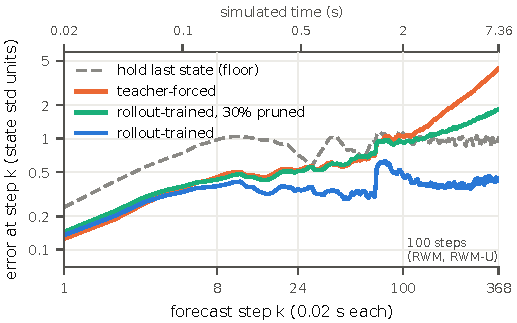
\includegraphics[width=\figw]{figures/fig_horizon.pdf}
\caption{Error at each forecast step on the 20 held-out trajectories of the five splits (models averaged within
each trajectory). All three simulators start together; teacher forcing first exceeds the floor (holding the last
state) at step {{fig_B_cross}}, and the 30\%-pruned copy, which starts within a few per cent of its parent, at step
{{fig_U_cross}}. Vertical lines: the imagination horizons of RWM and RWM-U.}
\label{fig:horizon}
\end{widefigure}

\textbf{Training objective.} Teacher forcing is trained on the one-step target and wins there: its one-step error
is {{ab_h1_pct_better}} lower than rollout training's on the 20 held-out trajectories ({{ab_h1_diff}} {{ab_h1_ci}}),
as an earlier registered analysis found on {{x3_h1_n}} short windows with the release's relative error
({{x3_h1_gap}} {{x3_h1_ci}}). By 8 steps the order has reversed on {{ab_h8_nworse}} of the 20 trajectories, and
the gap then grows with the horizon (Table~\ref{tab:decisions}, Fig.~\ref{fig:horizon}). At 368 steps a decision rule committed before the runs found the teacher-forced error
higher by {{x3_gap}} {{x3_ci}} in the release's relative error ({{x3_ratio}}$\times$; \textsc{{{x3_reading}}}), and
all {{x3_n_eps}} held-out episodes favour rollout training (sign test $p={}${{x3_p}}). In physical terms, over the first 2~s of imagined walking
the teacher-forced simulator's joint angles are off by {{ph_jdeg_h100_B}}$^\circ$ on average against
{{ph_jdeg_h100_A}}$^\circ$ for rollout training ({{ph_jdeg_h1_B}}$^\circ$ and {{ph_jdeg_h1_A}}$^\circ$ one step ahead), and over
7.4~s by {{ph_jdeg_h368_B}}$^\circ$ against {{ph_jdeg_h368_A}}$^\circ$. Dead-reckoned from the predicted velocities,
it misplaces the robot by {{ph_pos_h100_B}}~m after 2~s against {{ph_pos_h100_A}}~m (the robot covers
{{dist_h100}}~m), and by {{ph_pos_h368_B}} against {{ph_pos_h368_A}}~m after 7.4~s. For position over 2~s neither
beats extrapolating the last measured velocity ({{ph_pos_h100_floor}}~m); by 7.4~s rollout training does
({{ph_pos_h368_floor}}~m) and teacher forcing does not.

\textbf{Training horizon and stability.} With the history fixed at 32 steps, the model trained one step ahead
($N=1$) is the more accurate one step ahead (error ratio {{N1overN8_E1}} against $N=8$) and {{N1overN8_E100}} times
worse at 100 steps (Table~\ref{tab:decisions}); conversely the $N=32$ model has the highest one-step error of the
nine configurations ({{N32_E1}}) and the lowest 100-step error ({{N32_E100}}). The growth rate explains why: it is positive for $N=1$
({{N1_lam}}/s), so two copies of that simulator started a hair apart drift further apart, and it falls steadily as
the training horizon grows, through {{N2_lam}}, {{N8_lam}} and {{N16_lam}} to {{N32_lam}}/s at $N=32$; the sign
changes between two and eight steps. A rule committed before that analysis read Spearman's $\rho(N,\lambda_1)=$
{{ng_q4_rho}} {{ng_q4_ci}} over {{ng_q4_n}} models (\textsc{longer is more stable}). On the five splits,
every teacher-forced model has $\lambda_1>0$ and no rollout-trained one does.
Longer teacher-forced training makes this worse even as accuracy improves: from 500 to 10{,}000 iterations its
growth rate rises from {{ng_pathB_lam_500}} to {{ng_pathB_lam_10000}}/s while its 368-step error falls from
{{ng_pathB_E_2500}} (at 2{,}500) to {{ng_pathB_E_10000}}, whereas rollout-trained models become steadily more
stable ({{ng_pathA_lam_500}} to {{ng_pathA_lam_10000}}/s).

\textbf{Compression.} Setting the smallest 30\% of weights to zero without retraining keeps {{K_u30_h1}} of the
parent's skill one step ahead and {{K_u30_h24}} at 24 steps, but {{K_u30_h100}} at 100 steps and {{K_u30_h368}} at
368 steps: by the end it is worse than predicting no change (Fig.~\ref{fig:horizon}). Yet pruning barely moves the growth rate: 30\% pruning changes $\lambda_1$ by
{{lamshift_u30}}/s {{lamshift_u30_ci}} (registered: \textsc{{{q6_verdict}}}) and
none of the {{q6_nparents}} pruned copies has $\lambda_1>0$, so a pruned simulator is biased rather than
unstable (Sec.~\ref{sec:checks}). Pruning 20\% keeps {{K_u20_h1}} of the skill one step ahead and {{K_u20_h368}}
at 368 steps (Table~\ref{tab:decisions}). 8-bit weights keep {{K_int8w_h1}} of the skill one step ahead and {{K_int8w_h368}}
at 368 steps, and 16-bit weights {{K_fp16_h368}}. Removing units to width 192 fails at every horizon
({{K_s192_h1}} one step ahead) and needs fine-tuning. In a pre-registered test of PyTorch's 8-bit dynamic quantisation (weights
and activations; the release's relative error), the model kept {{perc_int8_K}} {{perc_int8_K_ci}} of its skill at
368 steps, and compiled with TorchScript it ran a one-robot step in {{perc_us_jit_int8}}~$\mu$s on a 2017 dual-core
laptop processor, {{perc_ratio_jit}} times the compiled 32-bit time; uncompiled, 8-bit was slower ({{perc_ratio_eager}}
times).

\textbf{Uncertainty.} The released five-head ensemble's spread ranks error well (Spearman {{dis_spear_h100}} with
the 100-step error) but is too small, by a factor that grows with the horizon (Table~\ref{tab:decisions}): a single
constant, which a penalty weight could absorb, cannot repair it. At 100 steps $\pm1\sigma$ covers {{cov1_h100}} of
outcomes against {{cov_nom1}} for a calibrated estimate. Two causes are structural. The five heads share
{{shared_pct}} of their parameters, one recurrent trunk, so they can disagree only about what it carries; rolling
each head out on its own predictions raises the 100-step coverage to {{cov1_h100_per}}. And each head's own
variance collapses, because the implemented loss is squared error on a prediction sampled from that variance,
whose expectation, $(\mu-y)^2+\sigma^2$, is smallest at $\sigma=0$: on synthetic data whose noise varies
{{synth_span}}-fold, the released head sits {{synth_under}}$\times$ below the true noise, while the authors' unused
likelihood loss recovers it (ratio {{synth_nll}}). A multiplier per horizon, fitted on nine episodes and scored on
the tenth, restores $\pm1\sigma$ coverage (\textsc{{{x7_summary}}}) but not the tails ($\pm2\sigma$:
{{cov2_perh_h100}} against {{cov_nom2}}). The released model's training rows are not recorded, so none of these is
a held-out measurement.

\subsection{Which check predicts error at the horizon of use?}\label{sec:checks}
A practitioner choosing among simulators, or deciding whether a compressed copy is fit to use, needs a check that
ranks them by their error at the horizon of use. We registered this comparison before running any model through the
code (Sec.~\ref{sec:setup}). The candidates were two labelled checks, the one-step error $E_1$ and the error over the
8-step training horizon $E_8$, both computed from every position of the held-out data; and two label-free checks
that use only the network, a recorded history and the commands, the growth rate $\lambda_1$ and the kinematic
residual $\bar r_J$. The target was $E_{100}$, the error over the 100-step horizon of RWM-U's imagined rollouts.

Table~\ref{tab:checks} and Fig.~\ref{fig:checks} give the result. Across the {{n_P}} simulators of F18, one-step
error ranked the 100-step error poorly (Spearman {{q1_rho_e1}}), the growth rate well ({{q1_rho_lam}}) and the 8-step
error about as well ({{q2_rho_e8}}). The first primary comparison favours the label-free check, $\lambda_1$ over $E_1$
by {{q1_delta}} {{q1_ci975}} (\textsc{{{q1_verdict}}}); the second cannot separate it from the 8-step error
({{q2_delta}} {{q2_ci975}}, \textsc{{{q2_verdict}}}). The same held at 368 steps; at 24 steps, which the 8-step windows
nearly cover, the 8-step error ranked ahead of the growth rate. Without the one-step-trained models ({{n_RC}} simulators) the
growth rate still ranked better than one-step error ({{q5_1_delta}} {{q5_1_ci}}). The kinematic residual, also label-free,
ranked best of all ({{q4_1_rho_new}}), ahead even of the 8-step error ({{q4_8_delta}} {{q4_8_ci}},
\textsc{{{q4_8_verdict}}}).

Where one-step error goes wrong is visible in Fig.~\ref{fig:checks}: the models trained one or two steps ahead have
among the lowest one-step errors and 100-step errors several times those of the best rollout-trained models. Split by what differs between the simulators
(exploratory), one-step error ranks the training choices backwards (Spearman {{x2_tc_E1}} {{x2_tc_E1_ci}} over the
{{x2_tc_n}} trained models of F18; {{x3_unc_E1}} within the five splits), while every check ranks the compressed
copies of one model well ({{x2_c_lam1}} to {{x2_c_E8}}). In practice, choosing among the nine training configurations
of each seed by one-step error picked a model trained one or two steps ahead for every seed, with a 100-step error {{regret_E1_ratio}} times the best available; choosing by the growth rate picked the
best configuration for {{n_pick_lam_best}} of the three seeds and came within {{regret_lam1}} of the best 100-step
error on average.

The registered replication on the five splits did not hold for the growth rate. There, where 40 of every
{{n_X_fold}} simulators are compressed copies, one-step error ranked better than the growth rate ({{q3_1_delta}}
{{q3_1_ci}}, \textsc{{{q3_1_verdict}}}) and the 8-step error better still ({{q3_8_rho_base}}). The reason is what the growth rate measures:
whether a simulator amplifies small differences. Moderate pruning makes a simulator biased, not unstable, so
$\lambda_1$ barely moves while the 100-step skill drains away (Sec.~\ref{sec:decisions}), and a negative growth rate
certifies nothing: of the {{d4_F18_worse_total}} F18 simulators worse than holding the last state at 100 steps,
{{d4_F18_non_worse}} had $\lambda_1\le0$. The authors' released model shows the converse: on its 20 trajectories,
which it may have trained on, its one-step error is low ({{rel_E1}}, against {{released_floor_E1}} for the floor),
yet its growth rate is positive ({{rel_lam}}/s) and over 368 steps its error exceeds the floor's ({{rel_E368}}
against {{released_floor_E368}}). The kinematic residual, registered on F18 only, also ranked the five-split pool
best (exploratory: {{x1_rJ}}, level with the 8-step error).

\begin{widetable}[t]
\centering
\caption{Which pre-deployment check ranks the 100-step error $E_{100}$? Spearman correlation across simulators (1 is
a perfect ranking, negative is backwards). Columns: the {{n_P}} simulators of F18 (4 held-out trajectories), split
(exploratory) into the {{x2_tc_n}} that differ in how they were trained and the {{x2_c_n}} compressed copies; and the
{{n_X}} simulators of the five splits (20 trajectories), correlated within each split and averaged. Below: the
registered comparisons, with 97.5\% intervals for the two primary ones and 95\% otherwise, from resampling
simulators (within splits on X5). E: exploratory.}
\label{tab:checks}
\footnotesize
\setlength{\tabcolsep}{4pt}
\fittable{\begin{tabular}{@{}lccccc@{}}
\toprule
 & Needs recorded & F18, all & F18, training & F18, & X5, five \\
Check & future states & ({{n_P}}) & choices ({{x2_tc_n}}, E) & compressed ({{x2_c_n}}, E) & splits ({{n_X}}) \\
\midrule
One-step error $E_1$ & yes & {{q1_rho_e1}} & {{x2_tc_E1}} & {{x2_c_E1}} & {{q3_1_rho_base}} \\
8-step error $E_8$ & yes & {{q2_rho_e8}} & {{x2_tc_E8}} & {{x2_c_E8}} & {{q3_8_rho_base}} \\
Growth rate $\lambda_1$ & no & {{q1_rho_lam}} & {{x2_tc_lam1}} & {{x2_c_lam1}} & {{q3_1_rho_new}} \\
Kinematic residual $\bar r_J$ & no & {{q4_1_rho_new}} & {{x2_tc_rJ}} & {{x2_c_rJ}} & {{x1_rJ}} (E) \\
\midrule
$\lambda_1$ minus $E_1$ & & {{q1_delta}} {{q1_ci975}} & & & {{q3_1_delta}} {{q3_1_ci}} \\
\quad verdict & & \textsc{{{q1_verdict}}} & & & \textsc{{{q3_1_verdict}}} \\
$\lambda_1$ minus $E_8$ & & {{q2_delta}} {{q2_ci975}} & & & {{q3_8_delta}} {{q3_8_ci}} \\
\quad verdict & & \textsc{{{q2_verdict}}} & & & \textsc{{{q3_8_verdict}}} \\
$\bar r_J$ minus $E_8$ & & {{q4_8_delta}} {{q4_8_ci}} & & & {{x1_rJ_minus_E8}} {{x1_rJ_minus_E8_ci}} (E) \\
\quad verdict & & \textsc{{{q4_8_verdict}}} & & & -- \\
\bottomrule
\end{tabular}}
\end{widetable}

\begin{widefigure}[t]
\centering
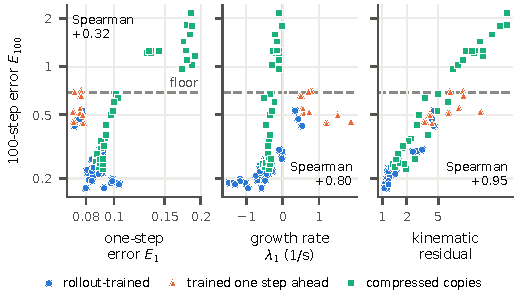
\includegraphics[width=\figw]{figures/fig_checks.pdf}
\caption{One-step error (left) and growth rate (right) against 100-step error for the {{n_P}} simulators of F18
(4 held-out trajectories). Models trained one or two steps ahead have among the lowest one-step errors but high
100-step errors, and positive growth rates. Compressed copies (squares) spread vertically at nearly constant growth
rate: pruning adds bias, not instability. Dashed: the floor, holding the last state.}
\label{fig:checks}
\end{widefigure}

\subsection{What label-free signals cannot do at run time}\label{sec:runtime}
A check that ranks whole simulators need not flag individual bad steps. Earlier analyses of these models, on
the same held-out trajectories of the five splits, found that none of the label-free signals is a usable alarm for a
step that is worse than holding the last state. On the rollout-trained ensembles, a combined kinematic-consistency
score reached an area under the ROC curve (AUROC; 0.5 is chance) of {{icp_auc_phys}} {{icp_auc_phys_ci}}, ensemble
disagreement {{icp_auc_dis}} and a plain step counter {{icp_auc_counter}}. Averaged over models of all three kinds, the growth
rate read step by step (over the last eight steps) reached {{ng_q3_auc}}, below the step counter's {{ng_q3_counter}}
(difference {{ng_q3_delta}} {{ng_q3_ci}}; registered: \textsc{worse than counter}). Re-synchronising the simulator with the recorded state when the
kinematic score fired gave {{icp_h7_excess}} {{icp_h7_ci}} more 368-step error than the same number of
re-synchronisations on a fixed schedule (registered: \textsc{schedule better}). Physics helps as a repair only where it is exact: rescaling the predicted
gravity direction to unit length changed the 368-step error by {{icp_G}} {{icp_G_ci}}, while forcing the joint
angles onto the approximate integration rule multiplied it by {{icp_J_x}}.

\section{Discussion}\label{sec:discussion}
\textbf{A checklist for vetting a learned robot simulator.} Every check below takes seconds per model on a
CPU.
(1)~\emph{Train for the horizon of use.} Training on the model's own rollouts, eight or more steps ahead here, gave
simulators that damp their own errors; one-step training gave simulators that amplify them, whatever their one-step
accuracy. (2)~\emph{Validate at the horizon of use}, on held-out episodes, counting independent trajectories rather
than overlapping windows: one-step and short-horizon scores mis-ranked the training objective and passed a pruned
model that has lost most of its skill by 2~s. (3)~\emph{Without recordings, check consistency and stability.} The kinematic residual matched or beat every
other check at ranking the 100-step error on both pools, at the cost of a few arithmetic operations per step; a positive growth rate flags a
simulator that amplifies its own errors, as one-step training produces, but a negative one certifies nothing, because
compression adds bias that it does not see. (4)~\emph{Read ensemble spread as a ranking}, and rescale it per horizon,
on held-out episodes, before using it as an interval. (5)~\emph{Do not rely on label-free run-time alarms};
re-synchronise with measurements on a schedule.

\textbf{Limitations.} All evidence comes from one robot, one trotting gait on flat ground and ten 20-second episodes
of simulated data, so ``held out'' means other velocity commands of the same gait. The held-out pair F18 has four
independent trajectories and the five splits twenty, which bounds every interval; correlations across models treat
models as independent although they share training data, so their intervals may be too narrow. No policy is trained,
so what a mis-ranked or miscalibrated simulator costs a controller is not measured. The growth rate is a finite-time
exponent in the network's own coordinates and depends on the start direction by tenths of 1/s; compressed copies
were not fine-tuned, and the 8-bit variant rounds weights only. The registered replication of the growth-rate
comparison failed on the five-split pool, and the kinematic residual's standing there is exploratory.

\section{Conclusion}\label{sec:conclusion}
A learned legged-robot simulator should be judged at the horizon at which it will be used. On one open
quadruped simulator, checks made one step ahead favoured teacher forcing, one-step training and a pruned model that
loses most of its skill by 2~s, and an uncertainty estimate whose shortfall grows with the horizon. Multi-step
validation fixes this when recordings exist. When they do not, the network itself can still be questioned: whether it
amplifies its own errors, which separated good training choices from bad ones, and whether its predicted joints move
as its predicted speeds say, which ranked simulators best of all here. Neither replaces a recording for catching
errors as they happen.

\section*{Reproducibility and use of AI tools}
Every number in this paper is generated from result files by scripts that refuse to build the paper if a value is
missing; the pre-registrations with their commit times, the code, the per-model results and an independent
re-computation of the registered statistics will be released with the final version. An AI assistant (Claude,
Anthropic), working under the author's direction, wrote analysis code, ran analyses and drafted text; the author is
responsible for the content.

\bibliographystyle{IEEEtran}
\bibliography{refs}
